% Template from the DPHPC course website

% IEEE standard conference template; to be used with:
%   spconf.sty  - LaTeX style file, and
%   IEEEbib.bst - IEEE bibliography style file.
% --------------------------------------------------------------------------

\documentclass[letterpaper]{article}
\usepackage{spconf,amsmath,amssymb,graphicx}
\usepackage[english]{babel}
\usepackage[utf8]{inputenc}
\usepackage{verbatim}		
\usepackage{epstopdf}
\usepackage[font=footnotesize]{caption}
\usepackage[dvipsnames]{xcolor}
\usepackage{hyperref}
\usepackage{listings}	
\usepackage{multicol}
\usepackage{ifthen}
\usepackage{tikz}
\usepackage{placeins}
\usetikzlibrary{arrows,decorations.pathmorphing,backgrounds,fit,positioning,shapes.symbols,chains,calc,shapes}

\usepackage[ruled,noend,noline,slide]{algorithm2e}
\newenvironment{listing}[1][htb]
  {\renewcommand{\algorithmcfname}{Listing}% Update algorithm name
   \begin{algorithm}[#1]%
  }{\end{algorithm}}

\usepackage{booktabs}
  
% Example definitions.
% --------------------
% Nice typeset for C++
\newcommand{\Cpp}{C\nolinebreak[4]\hspace{-.05em}\raisebox{.2ex}{\small \bf ++}}
%\newcommand{\Cpp}{C\nolinebreak\hspace{-.05em}\raisebox{.4ex}{\tiny\bf +}\nolinebreak\hspace{-.10em}\raisebox{.4ex}{\tiny\bf +}}
%\newcommand{\Cpp}{\texttt{C\nolinebreak+\nolinebreak+}}


% bold paragraph titles
\newcommand{\mypar}[1]{{\bf #1.}}

\ifthenelse{\boolean{false}}% TODO: change to false to hide invisible notes
{ \newenvironment{invisible}{\par\bigskip\color{gray}}{\par\bigskip} }%
{ \newenvironment{invisible}{\expandafter\comment}{\expandafter\endcomment} }

\title{Topological Sorting: A Parallel Implementation}

\name{J. Baum, K. Wallimann, M. Untergassmair}%
\address{ETH Zürich, HS 2015 \\
	Design of Parallel and High Performance Computing \\
	Zürich, Switzerland}

%%%%%%%%%%%%%%%%%%%%%%%%%%%%%%%%%%%%%%%%%%%%%%%%%%%%%%%%%%%%%%%%%%%%%%%%%%%%%%%%

\begin{document}

\maketitle

\begin{abstract}
	This short report gives a quick insight in topological sorting and the various problems that are associated with its parallelization.
	Building on existing algorithms, it suggests modified and optimized approaches to overcome these problems while making best use of state of the art computer hardware.
	In a discussion of the obtained benchmarks the performance of these approaches is analyzed and compared.
	Lastly, this report contains some suggestions regarding which graph types might profit from parallel topological sorting.
\end{abstract}

\section{Introduction}\label{sec:intro}

\mypar{Motivation}
\begin{invisible}
  \begin{itemize}
  \item Software Dependencies
  \item Maybe, to flesh out: Admittedly a bit academic, but interesting problem nevertheless, because memory bound => This is the future of HPC
  \end{itemize}
\end{invisible}


\mypar{Related work} 
\begin{invisible}
  \begin{itemize}
  \item MC Er Paper \cite{er1983parallel}: Unclear how to retrieve a sorted list from values without sorting and threads might chase other threads. No words about load balancing => Not practicable
  \item Ma Paper \cite{ma1997efficient}: Theoretical analysis in PRAM model, not practicable.
  \item Both cases: No code
  \item Our contribution: (1) Modified algorithm based on MC Er. 1. Sorted list is directly extracted. 2. only one thread continues when multiple threads meet. 3. Ensure load balancing
                          (2) Actual implementation for shared memory architecture
  \end{itemize}
\end{invisible}



\section{Algorithm}\label{sec:background}
%TODO: Johannes

 In this section, we define the topological sort problem and contrast it to Breadth-First-Search (BFS) and Depth-First-Search (DFS).
 Furthermore, we introduce the basics of the parallel algorithm we use.
 \\
 

\mypar{Topological sorting}
 A directed acyclic graph (DAG) describes a partial order. A topological sorting is a total order on a DAG. Let $G = (V,E)$ be a DAG where $V$ is the set of vertices and $E$ is the set of edges. Given $G$, a topological sorting is formally a function $ord: V \longrightarrow \{1,...,n\}$ where $n = |V|$ such that $\forall (v,w) \in E: ord(v) < ord(w)$ \cite[Chapter~9.1]{ottmann2012algorithmen}.

Figure \ref{fig:ts-example} shows a DAG for which one possible topological sorting is A,I,F,B,E,D,H,G,C. Every DAG has at least one topological sorting, but in general there are many different topological sortings for the same graph.

\begin{figure}[!hbp]
 \centering
  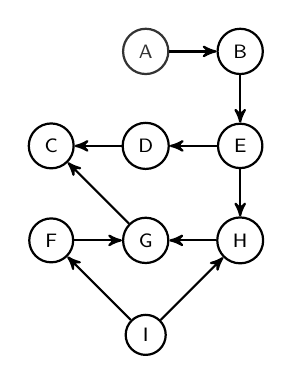
\begin{tikzpicture}[->,>=stealth',auto,node distance=1cm,
                    thick,main
                    node/.style={circle,draw,font=\sffamily\scriptsize},text node/.style={draw=none,font=\sffamily\tiny}]

  \node[main node] (1) [draw=black!80,text=black!80] {A};
  \node[main node] (3) [right of=1, node distance=1.2cm]{B};
  \node[main node] (7) [below of=3, node distance=1.2cm] {E};
  \node[main node] (4) [left of=7, node distance=1.2cm] {D};
  \node[main node] (5) [below of=7, node distance=1.2cm] {H};
  \node[main node] (6) [left of=4, node distance=1.2cm] {C};
  \node[main node] (8) [left of=5, node distance=1.2cm] {G};
  \node[main node] (9) [below of=8, node distance=1.2cm] {I};
  \node[main node] (2) [left of=8, node distance=1.2cm] {F};


  \path[every node/.style={font=\sffamily\small}]
    (1) edge (3)
    (3) edge (7)
    (7) edge (4)
    (4) edge (6)
    (7) edge (5)
    (5) edge (8)
    (8) edge (6)
    (9) edge (5)
    (9) edge (2)
    (2) edge (8)
    ;
\end{tikzpicture}

\caption{Example DAG where A,I,F,B,E,D,H,G,C is one possible topological sorting}
\label{fig:ts-example}
\end{figure}

Although the results of the breadth-first-search (BFS) algorithm seem to be similar to topological sortings, they are not equivalent. A topological sorting is a total order with respect to the partial order represented by the input graph. In contrast, the traversal sequences of a BFS (and DFS) generally don’t correspond to a total order induced by a DAG. A simple example is shown in figure \ref{fig:diff-bfs}. The visiting sequence A,C,B is a possible traversal sequence in BFS but is not a topological sorting. The only valid topological sorting for this graph is A,B,C.


\begin{figure}[!hbp]
\centering
 
  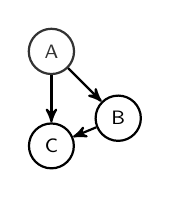
\begin{tikzpicture}[->,>=stealth',auto,node distance=1cm,
                    thick,main
                    node/.style={circle,draw,font=\sffamily\scriptsize},text node/.style={draw=none,font=\sffamily\tiny}]

  \node[main node] (1) [draw=black!80,text=black!80] {A};
  \node[main node] (2) [below right of=1, node distance=1.2cm]{B};
  \node[main node] (3) [below of=1, node distance=1.2cm] {C};
 

  \path[every node/.style={font=\sffamily\small}]
    (1) edge (2)
    (2) edge (3)
    (1) edge (3)
    ;
\end{tikzpicture}

\caption{A,C,B is a valid sequence in breadth-first-search (BFS) and depth-first-search (DFS) but not a topological sorting}
\label{fig:diff-bfs}
\end{figure}

Topological sorting has an asymptotic complexity of $\mathcal{O}(|V|+|E|)$ \cite[Chapter~22.4]{cormen2001introduction}. Sequential algorithms have been published by Kahn \cite{kahn1962topological} and by Tarjan  \cite{tarjan1976edge}. The latter is based on a DFS with backtracking.

 \mypar{Parallel algorithm}
 In 1983 M. C. Er \cite{er1983parallel} came up with a parallel approach to retrieve a topological sorting. The algorithm works in 5 steps:
 \begin{enumerate}
        \item Build the graph from the given partial order (optional if the problem is already stated as a graph).
        \item Add a special node value to every node and initialize it to zero
        \item Visit all source nodes (nodes with an indegree of zero) and set their node values to one.
        \item Let all source nodes be front nodes. For all child nodes of the front nodes, proceed in parallel as follows: Let $N_f$ be the node value of a front node and $N_c$ the node value of a child node. If $N_f \leq N_c$, the value of the child is set to $N_f + 1$. After all child nodes have been processed, denote all child nodes as the new front nodes. Repeat this step until there are no further child nodes. 
        \item List all the nodes in ascending order of node values.
 \end{enumerate}
 
To avoid a race condition by concurrent writes to a node’s value, M. C. Er proposes a synchronization after every iteration of step 4. Therefore, any two threads would write the same number to a node’s value, because the barrier ensures that all threads are in the same iteration. This comes at the price of a lower performance, but avoids locking the node's value. However, node values might be rewritten by multiple threads that "follow" each other. For example, in figure \ref{fig:ts-example}, nodes H, G and C could receive the values 2,3,4 initially, but would eventually be overwritten with the values 4,5,6

The asymptotic parallel runtime of the above algorithm is stated by M. C. Er as $\mathcal{O}(D_{max})$, where $D_{max}$ is defined as the maximum distance between a source node and a sink node. This runtime is hard to achieve in practice if one implements step 5 of the algorithm via sorting the nodes with respect to their values. It is not mentioned by M. C. Er how to create the result list of step 5.

\mypar{Improvements}
We propose not to use node values, but to directly put the node into the solution list. This avoids sorting the nodes by their value at the end. However, it must be made sure that no node is written more than once to the result list and race conditions while writing to the solution list must be avoided.

Furthermore, we introduce a parent counter to address the problem of several threads processing the same nodes. For each node, the parent counter is initialized to the number of parent nodes. During the algorithm each thread arriving at a node will decrease the counter by one. It will only process the node if the parent counter is zero. Thus a node will be processed only by the last arriving thread. Care has to be taken of the race condition while updating the parent counter.



 
 
 
 \begin{invisible}
 % Serial TS
 \mypar{Topological sorting}
 \begin{itemize}
  \item What is topological sort, difference to BFS
  \item Input: A set of dependencies (aka partial orders) of the form A $\rightarrow$ B ``A must come before B''
  \item Output: A sequence (aka total order) containing all nodes exactly once. All partial orders must be kept.
  \item Solution not unique
  \item Minimal Example: A->B, A->C, B->C. Valid BFS traversal order: A, C, B. Invalid for TS.
  \item TS can (serially) be solved with Kahn's algorithm \cite{kahn1962topological} or DFS and Backpropagation (Tarjan \cite{tarjan1976edge}). % See Wikipedia
        Note that TS is not equivalent to DFS, e.g. for A->B, B->C, A->D, D->E, DFS and Backpropagation yields A, B, C, D, E, but another valid TS is A, B, D, C, E
  \item Asymptotic runtime: O(|V| + |E|)
As an aside, don't talk about "the complexity of the algorithm.'' It's incorrect,
problems have a complexity, not algorithms.  
 \end{itemize}

 % Multithreaded TS
 \mypar{Parallel algorithm}
 \begin{itemize}
  \item Short overview over algorithm of MC Er
  \item Parallelization over child nodes
  \item His idea with barrier in each step such that even if the index is written by multiple threads, they write the same number => Avoid race condition at writing the index
  \item Our idea: Instead of writing an index, directly write to solution list. As a consequence, we have to make sure that node is written to solution only once. And of course there is a race condition on writing to solution list.
  \item Our idea: First, count (in parallel) how many parents each node has. Each time a node is visited, decrement counter and only write to solution if counter is zero. Of course, there is a race condition on the parent counter.
  \item 3 synchronization points (that is, bottlenecks): 1. Barrier after each level, 2. Lock solution list for appending new nodes, 3. Lock parent counter for decrementing it and checking if it is zero.
  \item Cost
 \end{itemize}

 
\end{invisible}
\section{Efficient parallel implementation}\label{sec:yourmethod}
In this section, the implementation of the parallel algorithm outlined above is presented.
Especially, we show how to ensure load balancing, how to efficiently append nodes to the solution list, how to efficiently decrement and check the parent counter, and a way to circumvent barriers.
\begin{invisible}
 Achtung! Falls Barriers gestrichen werden, streiche and a way to circumvent barriers.
\end{invisible}

\mypar{Parallelization and load balancing}
Parallelization is achieved by distributing the nodes in the front among the threads.
The front initially consists of all source nodes.
After all front nodes have been processed, all their child nodes are added to the front while the former front nodes are removed from the front.
If there are no more child nodes, all nodes have been processed and the algorithm terminates.
We experimented with three different implementations to achieve parallelization and load balancing.

Firstly, the \emph{``Scatter-Gather''} implementation, represents the front using a linked list of node (pointers). Initially, the source nodes are inserted into this list.
Following an idea described in \cite{bulucc2011parallel}, the nodes in the front are scattered among the threads, such that each thread owns a thread-local list,
that represents its share of the nodes in the front.
Child nodes for the next front are first inserted to another thread-local list.
When the whole front was processed, one thread gathers all thread-local lists and redistributes the new child nodes among the threads.
Redistribution for each front already yields some level of load balancing.

Secondly, the \emph{``Worksteal''} implementation further refines load balancing using a work stealing policy.
If one thread runs out of nodes within a front (i.e. the thread-local node list is empty), it can steal nodes from another thread that has not finished yet. In our implementation we randomly select the thread from which to steal.

Thirdly, the \emph{``Node-Lookup''} implementation represents the front using an array of boolean flags, as used in the context of BFS in \cite{agarwal2010scalable} or \cite{beamer2013direction}. The size of the flag-array is equal to the number of nodes.
The last parent visiting a child node sets the child nodes' flag to true. Parallelization is then enabled by parallelizing the loop over the array.
Load balancing is conveniently achieved using a dynamic scheduler.
Notice that we cannot use a space-efficient bitset for the parallel implementation, because is not thread-safe.

\mypar{Appending to the solution list}
%All nodes in the current front have already been visited by all their parent nodes. % This is actually an invariant, but never mind.
%This is ensured by admitting only those child nodes to the next front, for which the current node is the last visiting parent node. % Maybe belongs to algorithm description
Nodes can be added to the global solution list, if they are in the current front.
The order among the nodes on one front does not matter for the topological sorting:
By construction of our algorithm, the front only contains nodes that have already been visited by all their parents (parent counter). Thus, one node cannot be parent of another node in the current front.
As a consequence, the nodes can be appended to the solution concurrently without any restrictions on the order.
Still, the solution list has to be locked for every appending of a node, which is not optimal.

The optimization that we propose here is simple: Every thread first inserts the nodes in a thread-local list and then appends the whole local list to the solution list.
Thereby, each thread grabs the lock only once per front and not for every node individually.
For lists, appending another list can be done in constant time.

\mypar{Decrementing and checking the parent counter}
In the parallel algorithm, every node has a parent counter that is initialized with the number of parent nodes.
As explained before, a node may only be inserted if all its parents have visited it.
Therefore, each parent has to decrement the parent counter to mark its visit and it has to check whether the parent counter is zero, i.e. whether it is the last visiting parent.
Na{\"i}vely, the decrement and the check have to be locked together, in order to avoid race conditions on the counter on the one hand, and in order to ensure that only one thread may return true on the other hand. 
However, a closer examination reveals that these requirements can be met by using atomic operations.

\begin{listing}
 \SetKw{KwRet}{Return}
 \SetKw{KwBool}{Bool}
 \SetKw{KwInt}{Integer}
 \SetKwProg{Fn}{Function}{}{}
  \KwInt parentCounter\;
  \tcp{initialized with number of parent nodes}
  \KwBool token = false\;
  \Fn{decrementAndCheckParentCounter{}} {
    AtomicDecrement(parentCounter)\;
    \KwBool swapped = false\;
    \If{parentCounter == 0}{
      swapped = AtomicCompareAndSwap(token, false, true)\;
    }
    \KwRet swapped;
  }
 \caption{Efficiently decrementing and checking the parent counter using atomic operations.}
 \label{lst:parentCounter}
\end{listing}

Listing \ref{lst:parentCounter} shows the implementation using two separate atomic operations. Multiple threads may in fact decrement the counter before the function returns.
However the atomic compare-and-swap ensures that only one thread can return true. This is important if the current front is implemented as a list.
In this case, the child node would be inserted twice, if multiple threads returned true, which is wrong.
If the front is implemented as an array of flags, the compare-and-swap is in fact not necessary, because it makes no difference if multiple threads set the flag.

\mypar{Barrier-free implementation}
Barriers are used to process the nodes in a front-by-front fashion.
Each front is finished with a barrier, either explicitly, if the front was implemented with a list, or implicitly by a for-loop, if the front was implemented using a array of flags.

If barriers are given up, it is no longer certain that all threads work on nodes of the same front.
Some threads may already work on nodes of the next front, while other threads are still working on the previous front.

A priori, this is not a problem, because in any case, a node is only appended to the solution list if all its parents have visited it, regardless of which front its parents belonged to.
However, it is not possible to temporarily store a node in a thread-local list and defer the appending to the solution list, as suggested earlier.
In this case, it would be possible that a node was appended to the solution list, while its parent node has only been appended to a thread-local list, but not yet to the solution list, leading to an invalid result.

Hence, avoiding barriers seems to be a trade-off between the cost of barriers and the cost of locking the solution list for every node.

\begin{invisible}
Hmm... we could defer decrementing the parent counter and inserting the child node until the local list is appended to the solution list. That means, that we have to touch all nodes twice
Somewhere, we need to mention that we are working with an adjacency list.
\end{invisible}

\section{Experimental Results}\label{sec:exp}
%
In this section, we present our experimental setup and the impact of the different optimizations and implementations described in the previous section.
\par\medskip
%
\mypar{General note about the presented plots}
In all the plots that are presented in this section the marker symbol locates the mean of each measurement while the variance of the data is shown as a probability density around that mean value.
For the computation of the speedup on $n$ threads defined as $t_1/t_n$ the mean value of the one-threaded timing $t_1$ of the parallel code was used.
A list of these single-threaded timings can be found in table \ref{tab:t1timings}. 
\par\medskip
{\Large TODO: timing table}
\par\medskip
(the 95\% confidence interval of each set of measurements of $t_1$ is less than $\pm 10\%$ around the mean). \\
The discussion in this paper will focus on the topological sorting of a random graph with average node degree 32 and a base size of 1Mio nodes.\footnote{All plots in this section refer to graphs with 1Mio nodes except for the weak scaling graphs where the base size is 1Mio and the effective size in each execution is given by number~of~threads~$\times$~1Mio} 
While the speedup of our algorithms highly depend on the graph type (and in particular on its density), the relative positioning of different optimization strategies is consistent between all the graphs that were tested. \\
For a more comprehensive overview with more detailed scaling plots we refer to the projects Git repository (see link below).
\par\medskip

%%%%%%%%%%%%%%%%%%%%%%%%%%%%%%%%%%%%%%%%%%%%%%%%%%%%%%%%%%%%%%%%%
% HARDWARE AND COMPILER
%%%%%%%%%%%%%%%%%%%%%%%%%%%%%%%%%%%%%%%%%%%%%%%%%%%%%%%%%%%%%%%%%
\mypar{Hardware and compiler}
  \begin{table}[h]
    \centering
    \begin{tabular}{ll}
    \toprule
    Processor        & Intel Xeon E5-2697 (Ivy bridge) \\
    Max. clock rate  & 3.5 GHz (with TurboBoost)\\
    \# Sockets       & 2 \\
    Cores / socket   & 12 \\
    Threads / socket & 24 \\
    LLC / socket     & 30 MB \\
    \midrule
    Compiler and flags & GCC 4.8.2, -O3\\
    \bottomrule
    \end{tabular}
    \caption{Hardware and compiler used for benchmarks}
    \label{tab:hardware}
  \end{table}
 
The following experiments were run on a 24-core system consisting of 2 Intel Xeon E5 processors (see table \ref{tab:hardware}).
Hyperthreading was not used for the benchmarks.
The implementations were written in \Cpp, using OpenMP and GCC atomic built-in functions. The graph was stored in an adjacency list.
\par\medskip



\mypar{Effect of Optimization Strategies}
How does the initial, naive code compare to code that was enhanced with the Node-Lookup, Worksteal and other optimizations?
Figure \ref{fig:abstiming} shows the absolute timing of all the different algorithms that were implemented in this project.
{\Large TODO: which ones give speedup, which ones don't?}
%
\begin{figure}[ht]
	\centering
	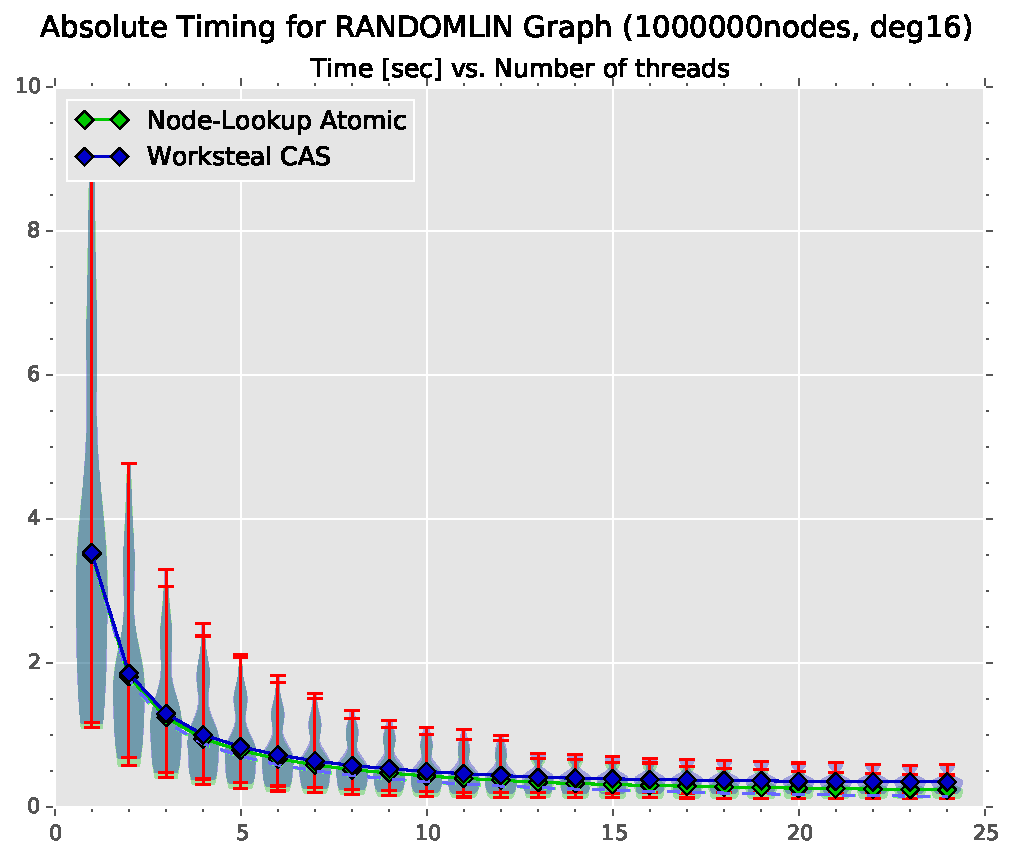
\includegraphics[width=\columnwidth]{plots/abstiming_gtRANDOMLIN_n1000000_deg16.pdf}
	\caption{<+caption text+>}
	\label{fig:abstiming}
\end{figure}
\par\medskip

%%%%%%%%%%%%%%%%%%%%%%%%%%%%%%%%%%%%%%%%%%%%%%%%%%%%%%%%%%%%%%
% BENCHMARKS
%%%%%%%%%%%%%%%%%%%%%%%%%%%%%%%%%%%%%%%%%%%%%%%%%%%%%%%%%%%%%%

\mypar{Benchmarks of Optimization Strategies}
So far we have seen that the Node-Lookup and Worksteal algorithms do in fact allow us to speed up the topological sorting by using multiple threads.
Next we want to look at the scaling behavior of the optimized algorithms to see which ones perform better. \\
The weak and strong scaling plots are shown in figure \ref{fig:weakscaling} and \ref{fig:strongscaling} respectively.

\begin{figure}[ht]
	\centering
	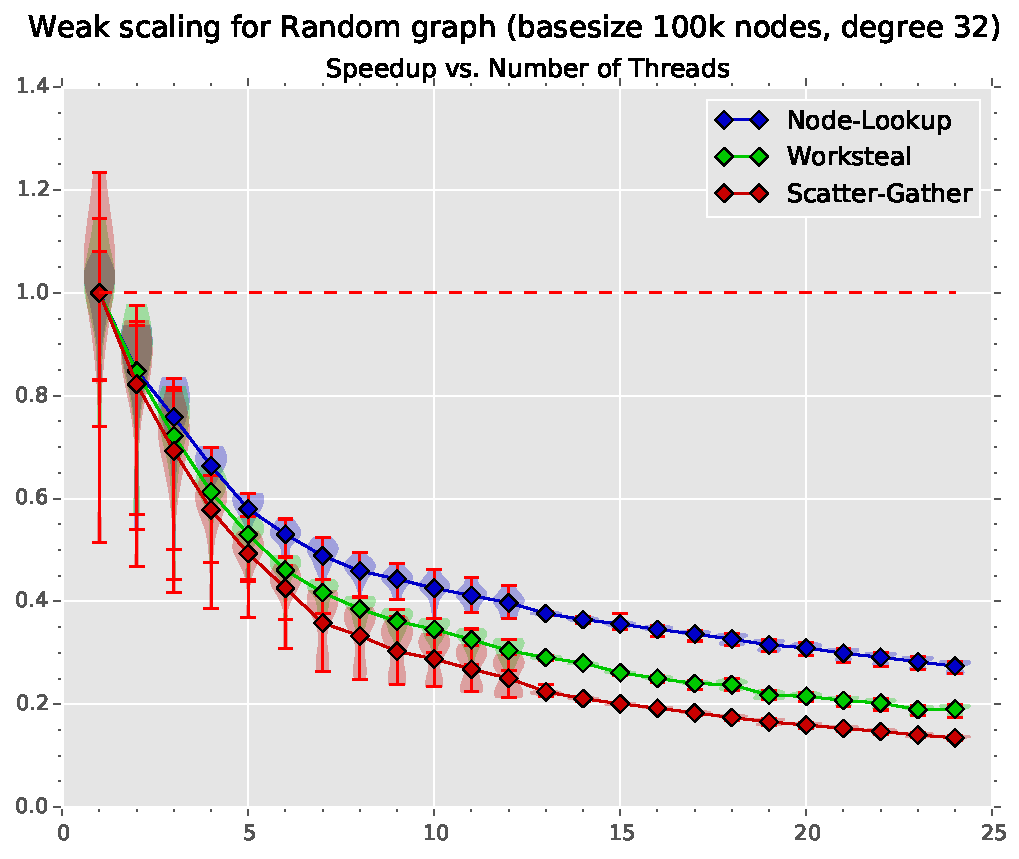
\includegraphics[width=\columnwidth]{plots/weakscaling_gtRANDOMLIN32_n1000000_deg32.pdf}
	\caption{The base size of the graphs in this weak scaling plot is 1Mio nodes.
		The Node-Lookup algorithm achieves the best performance and is only roughly 3 times slower at sorting a 24Mio node graph on 24 threads than in the base case. The Worksteal implementation takes approx. 5 times longer than the base case. \\
	It can also be noted that there is a relatively high speedup drop between 12 and 13 threads.
	This can be explained by the hardware on which the program is run. In fact, there are 24 cores but only 12 of them are on the same socket.
	Also the variance of the timings almost vanishes thread numbers higher than 12.
}
	\label{fig:weakscaling}
\end{figure}

\begin{figure}[ht]
	\centering
	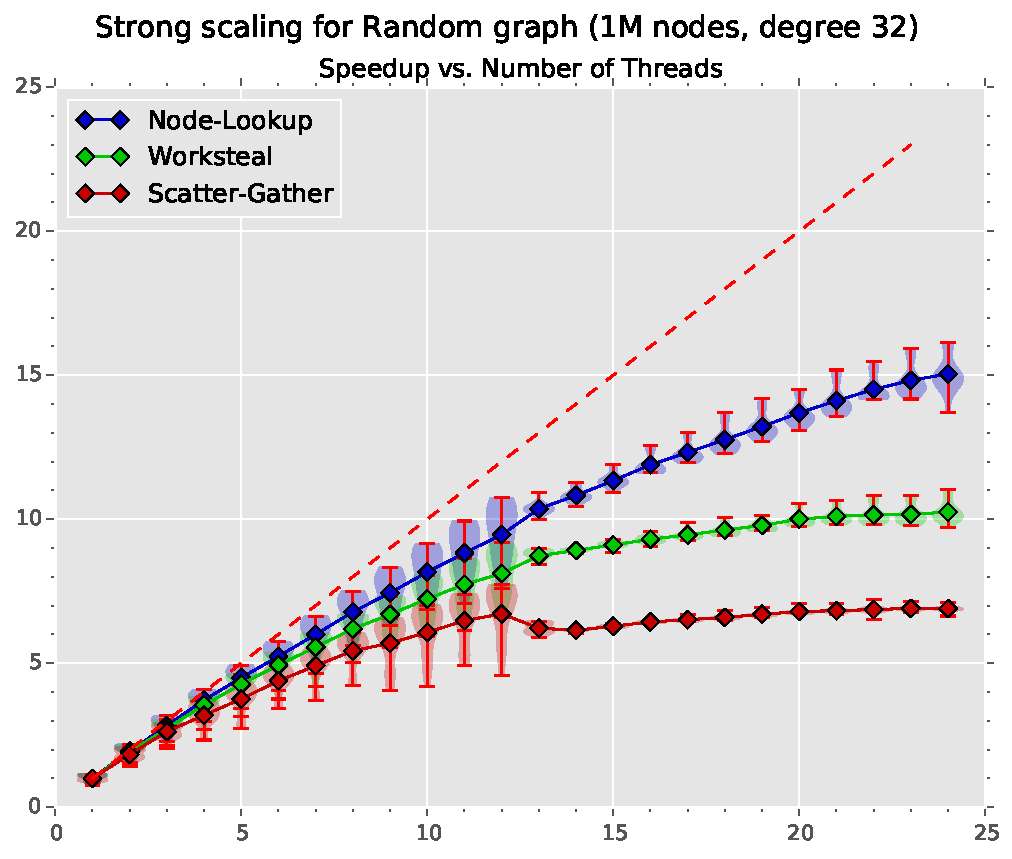
\includegraphics[width=\columnwidth]{plots/strongscaling_gtRANDOMLIN_n1000000_deg32.pdf}
	\caption{<+caption text+>}
	\label{fig:strongscaling}
\end{figure}




\begin{invisible}

 Strong Scaling software graph 

\end{invisible}


%%%%%%%%%%%%%%%%%%%%%%%%%%%%%%%%%%%%%%%%%%%%%%%%%%%%%%%%%%%%%%%%%
% GRAPH TYPES
%%%%%%%%%%%%%%%%%%%%%%%%%%%%%%%%%%%%%%%%%%%%%%%%%%%%%%%%%%%%%%%%%
\mypar{Dependency on Graph Type} As mentioned in the introduction to this section, we chose to focus our analysis to a random graph of node degree 32.
	For a 
%
\begin{figure}[ht]
	\centering
	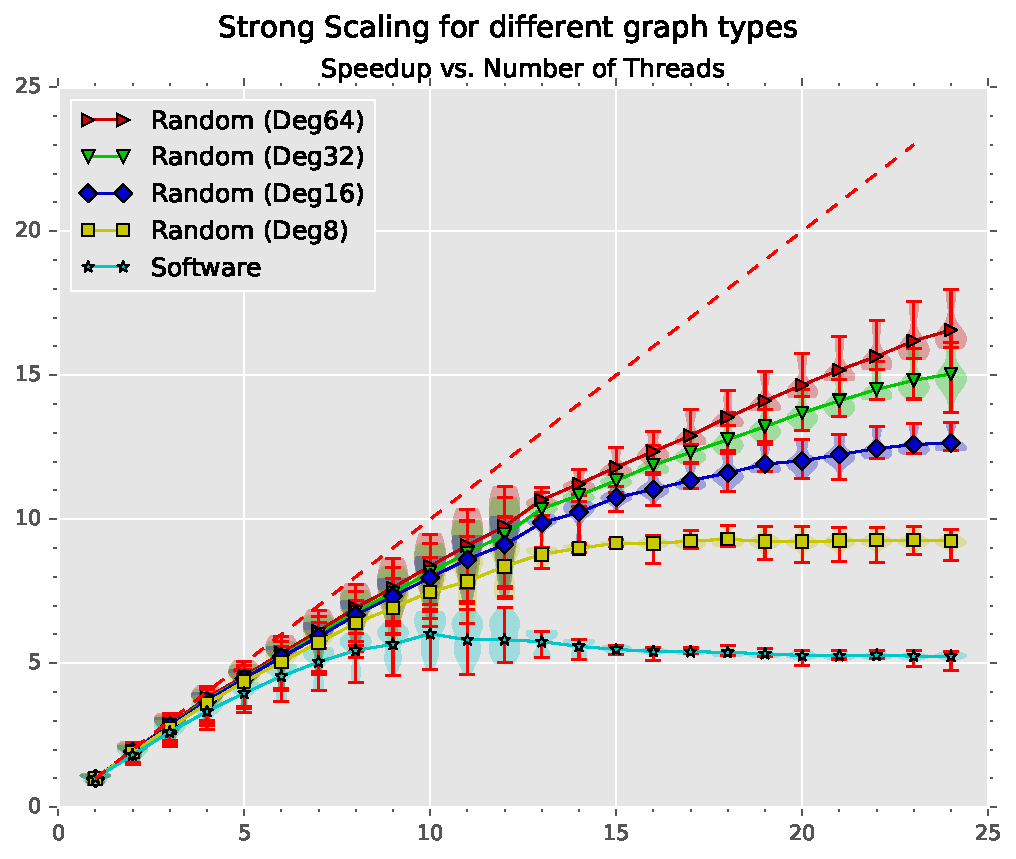
\includegraphics[width=\columnwidth]{plots/strongscaling_gtALL_n1000000.pdf}
	\caption{Strong scaling of the Node-Lookup algorithm for several different input graphs of size 1Mio nodes. The scaling is better for random graphs with higher node degree than for those with low node degree.
		The software graph (average node degree approx. 2) achieves a speedup of roughly 6x on 10 threads but does not scale any further.
}
	\label{fig:strongscaling_graphtypes}
\end{figure}
%
Figure \ref{fig:strongscaling_graphtypes} shows the strong scaling of the Node-Lookup algorithm for several different input graphs.
It should be noted that all of the analyzed graphs are artificial (i.e. they do not come from real-world datasets but are rather constructed to meet some requirements).
However, the construction of the software graph was done according to the description in \cite{musco2014generative} and should to some extend be a realistic emulation of a real world software graph. \\
However, the average node degree in such a software graph is very low meaning that the overhead required to synchronize the threads becomes large compared to the work that needs to be performed which in turn destroys most of the parallelism. \\
In fact, figure \ref{fig:strongscaling_graphtypes} clearly shows how the scaling behavior of the algorithm gets better for graphs that have more edges per node.
Nevertheless, even the random graph with average mode degree 32 that we used for our performance analysis is sparse since the number of edges $|E|$ in the graph is clearly much smaller than the maximum possible number of vertices $|V|(|V|-1)$ (in particular that the number of edges in the graph scale linearly with the graph size, $|E| \sim \mathcal{O} ( |V| )$). \\
Although the analyzed graphs are somewhat artificial, the performance analysis that was carried out in this report should still be a good indicator of how the topological sorting algorithms would scale on real-world graphs with similar densities.
To this point however, the performance of the algorithms on real-world graphs was not tested yet, and an investigation of such could be content of further research.
\par\medskip
%
Plots for other graph types can be found in the repository of our project which is listed at the end of this report.
\par\medskip

\section{Conclusion}
%
In this report we have extended the theoretical considerations made in \cite{er1983parallel} and discussed as well as tested its parallel implementation.
Both the Worksteal and the Node-Lookup approach can be considered successful parallelizations of the topological sorting algorithm, with the latter showing better absolute timings and scaling behavior for the graphs that were analyzed. \\
Finally, one main finding of this project is that the efficiency of the parallelization highly depends on the graph type: if the graph is too sparse and each node has only very few outgoing edges, then the parallelizable portion of the algorithm shrinks and by Amdahl's law the synchronization overhead dominates the runtime resulting in bad scaling. \\

\begin{invisible}
 \begin{itemize}
   \item Best thing would be to have no barriers and still local solution update
   \item Since this is not possible, it is better to accept barriers so as to benefit from local solution
   \item It is worth noting that performance highly depends on the structure of the graph.
 \end{itemize}
\end{invisible}


\section{Additional material}
%
The source code of the project, a database containing all the raw data that was collected for the benchmarking plots as well as many more detailed plots depicting the scaling behavior for all tested graph types can be found in the following Git repository:
\begin{center}
	\href{https://github.com/walkevin/ParallelTopologicalSorting.git}{https://github.com/walkevin/ParallelTopologicalSorting.git}
\end{center}


\bibliographystyle{IEEEbib}
\bibliography{bibliography}

\end{document}
